% !TEX root = ../stability.tex

\section{Real projective spaces}\label{s:continuous}

In this section ...

\subsection{Metric models}

For any integer $n\geq 1$ and real number $r>0$, let $\bbS^n(r)$ be the $n$-sphere of radius $r$, equipped with the geodesic distance.
The real projective space $\rp^n(r)$ is the quotient space $\bbS^n(r)$ by the antipodal map $x \mapsto -x$ for all $x \in \bbS^n$.
Let $[x]$ denote the equivalence class of $x$. We equip $\rp^n(r)$ with the quotient metric defined as
\[
d_{\rp^n(r)}([x],[x'])\defeq\min \{d_{\bbS^n(r)}(x,x'),d_{\bbS^n(r)}(-x,x')\}.
\]
For the simplicity of notation, let $\bbS^n\defeq\bbS^n(1)$ and $\rp^n\defeq\rp^n(2)$, so that $\diam\left(\bbS^n \right)=\diam\left(\rp^n \right)=\pi.$
It is proved in \cite{katz1983filling} that for any $n \geq 1$ their filling radius, as defined in \cref{ss:filling_radius}, satisfy
\[
\fillrad{\bbS^n} = \frac{1}{2}\arccos\left(\frac{-1}{n+1}\right), \qquad \fillrad{\rp^n}=\frac{\pi}{3}.
\]
We denote by $\zeta_n$ twice the filling radius of $\bbS^n$, i.e., $\zeta_n \defeq \arccos\left(\frac{-1}{n+1}\right)$.

\subsection{Vietoris--Rips homotopy types}

We recall the following results related to the homotopy type of the Vietoris--Rips complex of spheres and projective spaces.

\begin{proposition}
	Let $n$ be a positive integer.
	\begin{enumerate}[{\rm (a)}]
		\item\label{prop:S1}{\rm \cite[Thm.~7.4]{adamaszek2017vietoris}.}
		For $t \in \left(\frac{2l\pi}{2l+1}, \frac{2(l+1)\pi}{2l+3}\right]$
		\[
		\VR_t(\bbS^1) \simeq \bbS^{2l+1}.
		\]

		\item\label{prop:Sn}{\rm \cite[Thm.~10]{lim2020vietoris}.}
		For $t \in \left(0, \zeta_n\right]$
		\[
		\VR_t(\bbS^n) \simeq \bbS^n.
		\]

		\item\label{prop:RPn}{\rm \cite[Thm.~4.5]{adams2022metric}.}
		For $t \in \left(0,\frac{2\pi}{3} \right]$
		\[
		\VR_t(\rp^n) \simeq \rp^n.
		\]
	\end{enumerate}
	\anibal{Maybe unify $l$ and $n$.}
\end{proposition}

\subsection{Fundamental bars of $\VR_\bullet(\rp^n)$}

\begin{lemma} \label{prop:RPn bar}
	For integers $1 \leq p \leq n$,
	\[
	\left(0, \frac{2\pi}{3}\right) \in \Hbarc{p}{\rp^n}.
	\]
\end{lemma}

\begin{proof}
	We will use an induction argument on $n$.
	When $n = 1$, \cref{prop:manifold} implies that
	\[
	(0, 2\fillrad{\rp^1}) = \left(0, \frac{2\pi}{3}\right) \in \Hbarc{1}{\rp^1}.
	\]
	Assume the statement holds for $\rp^{n-1}$.
	That is, for any $1 \leq p \leq n-1$,
	\[
	\left(0, \frac{2\pi}{3}\right) \in \Hbarc{p}{\rp^{n-1}}.
	\]
	Let $t, \epsilon > 0$ be small.
	We claim that the following diagram of topological spaces commutes:
	\begin{equation}\label{d:fundamental_bars_diagram}
		\begin{tikzcd}
			\rp^{n-1}
			\ar[d, hook,"{\iota}" left]
			&
			\VR_t(\rp^{n-1})
			\ar[d, hook,"\iota_t"]
			\ar[l, "\rho_{n-1}" above, "\simeq" below]
			\ar[r, hook]
			&
			\VR_{\frac{2\pi}{3}+\epsilon}(\rp^{n-1})
			\ar[d, hook]
			\\
			\rp^{n}
			&
			\VR_t(\rp^{n})
			\ar[l, "\rho_n" below, "\simeq" above]
			\ar[r, hook]
			&
			\VR_{\frac{2\pi}{3}+\epsilon}(\rp^{n}).
		\end{tikzcd}
	\end{equation}
	In the above diagram, the horizontal inclusions are induced by the Vietoris--Rips filtration, whereas the vertical maps are induced by the equatorial inclusion of real projective spaces $\iota \colon \rp^{n-1} \hookrightarrow \rp^{n}$.
	It is therefore clear that the right square of \eqref{d:fundamental_bars_diagram} commutes.

	We now construct the remaining two maps $\rho_{n-1}$ and $\rho_{n}$ as in \cite[\textsection 4.3]{adams2022metric}.
	Let $f_n$ be the composition
	\[
	f_n \colon \VR_t(\bbS^n) \to \R^{n+1} \setminus \{0\} \xrightarrow{\pi_n} \bbS^{n},
	\]
	where the first map sends a formal linear sum $\sum_{i=1}^k \lambda_i x_i$ in $\VR_t(\bbS^n)$ to the sum $\sum_{i=1}^k \lambda_i x_i\in \bbR^{n+1}$ where $x_i\in \bbS^{n}$ and $\lambda_i\in \bbR$, and the second map $\pi_n$ is the radial projection map.\anibal{How are points in the VR cpx represented by formal sum? Probably this will be address in \cref{ss:vietoris-rips}}
	Because $f_n$ preserves the equivalence relation $x\sim -x$, we have the induced map \anibal{Maybe use superscripts for these maps and the $\rho$ too?}
	\[
	f_n/\sim:\VR_t(\bbS^{n})/\sim\to \bbS^{n}/\sim\cong \rp^n.\]
	Because $t<\frac{2\pi}{3}$, it follows from \cite[Lemma 4.4]{adams2022metric} that the map
	\[
	\alpha_n \colon \VR_t(\rp^n)\to \VR_t(\bbS^n)/\sim \text{ with }
	\sum_{i=1}^k \lambda_i [x_i]\mapsto \left[\sum_{i=1}^k \lambda_i x_i\right]
	\]
	is a homeomorphism, where $x_i\in \bbS^{n}$, $\lambda_i\in \bbR$, and $[\cdot]$ denotes the equivalence class of an element under the relation $x\sim -x$. We define
	\[\rho_n\defeq f_n/\sim \circ\,\alpha_n\]
	It is shown in \cite[Theorem 4.5]{adams2022metric} that $\rho_n$ is a homotopy equivalence from $\VR_t(\rp^n)$ to $\rp^n$ for any $n$.
	% In summary, we have defined the map
	% \[\rho_n: \VR_t(\rp^n)\xrightarrow{\cong} \VR_t(\bbS^n)/\sim\to \bbS^{n}/\sim\cong \rp^n\]

	We claim that the left square in the previous diagram commutes, i.e. $\iota\circ \rho_{n-1}=\rho_{n}\circ\iota_t$. Indeed, for any $y=\sum_{i=1}^k \lambda_i [x_i]\in \VR_t(\rp^{n-1})$, we have
	\begin{center}
		$(\iota\circ \rho_{n-1})(y)
		=\iota\left(f_{n-1}/\sim\left(\left[\sum_i \lambda_i x_i\right]\right)\right)
		=\iota\left(\left[f_{n-1}\left(\sum_i \lambda_i x_i\right)\right]\right)
		=\left[\pi_{n-1}\left(\sum_i \lambda_i x_i\right)\right]
		$
	\end{center}
	as an element in $\rp^n$, and
	\begin{center}
		$(\rho_{n}\circ\iota_t)(y)=\rho_{n}(y)=f_{n}/\sim\left(\left[\sum_i \lambda_i x_i\right]\right)=\left[f_{n}\left(\sum_{i=1}^k \lambda_i x_i\right)\right]=\left[\pi_{n}\left(\sum_{i=1}^k \lambda_i x_i\right)\right]
		$
	\end{center}
	Because $\pi_{n}$ restricted to $\rp^{n-1}$ is equal to $\pi_{n-1}$, we conclude that $(\iota\circ \rho_{n-1})(y)=(\rho_n\circ\iota_t)(y)$ for any $y$. Thus, the claim holds.\\

	For each $1\leq p\leq n-1$, applying the $p$-th homology functor (over $\Ftwo$) to the above diagram, we obtain the following commutative diagram of vector spaces:
	\[\begin{tikzcd}
		\mathrm{H}_p\left(\rp^{n-1}\right)
		\ar[d, "\cong" left]
		&
		\mathrm{H}_p\left(\VR_t(\rp^{n-1})\right)
		\ar[d, "\mathrm{H}_p(\iota_t)" left, "\cong" right, myred]
		\ar[l, "\cong" above]
		\ar[r, "g_{n-1}=0", myred]
		&
		\mathrm{H}_p\left(\VR_{\frac{2\pi}{3}+\epsilon}(\rp^{n-1})\right)
		\ar[d]
		\\
		\mathrm{H}_p\left(\rp^{n}\right)
		&
		\mathrm{H}_p\left(\VR_t(\rp^{n})\right)
		\ar[l, "\cong"]
		\ar[r, "g_n" , myred]
		&
		\mathrm{H}_p\left(\VR_{\frac{2\pi}{3}+\epsilon}(\rp^{n})\right).
	\end{tikzcd}\]
	By induction assumption, $\left(0, \frac{2\pi}{3}\right)\in\Hbarc{p}{\rp^{n-1}}$, which implies that $g_{n-1}$ is the zero map. Commutativity of the left-hand side square further implies that $\mathrm{H}_p(\iota_t)$ is an isomorphism. Then, using the right-hand side square's commutativity, we deduce $g_n\circ \mathrm{H}_p(\iota_t)=0$. Since $\mathrm{H}_p(\iota_t)$ is an isomorphism, we conclude that $g_n=0$. This holds for any $\epsilon>0$, so we can conclude $\left(0, \frac{2\pi}{3}\right)\in\Hbarc{p}{\rp^{n}}$.

	For the case when $p=n$, we can apply Item (\ref{prop:manifold}) to observe that $(0,2\fillrad{\rp^n}) = \left(0, \frac{2\pi}{3}\right)\in \Hbarc{n}{\rp^n}$. Therefore, $\left(0, \frac{2\pi}{3}\right)\in \Hbarc{p}{\rp^n}$ is established for all $1\leq p\leq n.$
\end{proof}

\subsection{Barcodes and Steenrod barcodes of $\bbS^n$}\label{ex:Sn}
Because the Vietoris--Rips complexes of $\bbS^n$ are contractible when the scale parameter $t>\pi$, neither the standard barcodes nor the Steenrod barcodes can stay alive after $\pi$. Therefore, all bars are dominated by $(0,\pi)$.

First, consider the case of $n=1$.
The barcodes of $\bbS^1$ can be obtained from Proposition \ref{prop:homotopy type} (\ref{prop:S1}), i.e. \cite[Theorem 7.4]{adamaszek2017vietoris}: for any $l\in \Z_{\geq 0}$,
\begin{equation}\label{eq:barc of S1}
	\Hbarc{2l+1}{\bbS^1}=\left\{\left(\tfrac{2l\pi}{2l+1},\tfrac{2(l+1)\pi}{2l+3}\right)\right\},\, \Hbarc{2l}{\bbS^1}=\emptyset.
\end{equation}
For $n\geq 2$, we have the following (see Figure \ref{fig:Sk}):
\begin{itemize}
	\item $\Hbarc{1}{\bbS^n}=\emptyset$, by \cref{prop:homotopy type} \cref{prop:pH1}.
	%\facundo{(VR-PH1 of any geodesic metric space is trivial. See papers by Virk. ( The Claim also follows from your own work on persistent homotopy groups.))}
	\item $\Hbarc{n}{\bbS^n}$ consists of one bar $(0,\zeta_n)$ (by Proposition \ref{prop:homotopy type} (\ref{prop:manifold})) and possibly some bars dominated by $(\zeta_n,\pi)$ (by Proposition \ref{prop:homotopy type} (\ref{prop:Sn})).
	\item For any degree $p\geq 2$ and $p\neq n$, the only possible bars in $\Hbarc{p}{\bbS^n}$ are those  dominated by  $(\zeta_n,\pi)$. This follows from  Proposition \ref{prop:homotopy type} (\ref{prop:Sn}).
\end{itemize}

\begin{figure}[ht]
	\centering
	\begin{tabular}{ c c  }
		\begin{tikzpicture}[scale=0.6]
			\begin{axis} [
				title = {\LARGE $\Hbarc{n}{\bbS^n}$},
				ticklabel style = {font=\Large},
				axis y line=middle,
				axis x line=middle,
				ytick={0.5,0.57,0.67,0.95},
				yticklabels={,$\zeta_n$,,$\pi$},
				xtick={0.5,0.57,0.95},
				xticklabels={$\frac{\pi}{2}$,$\zeta_n$, $\pi$},
				xmin=-0.015, xmax=1.1,
				ymin=0, ymax=1.1,]
				\addplot [thick,color=black!20!white,fill=black!30!white,
				fill opacity=0.4]coordinates {
					(0.57,0.95)
					(0.57,0.57)
					(0.95,0.95)
					(0.57,0.95)};
				\addplot [black!40!white,mark=none,dashed, thin] coordinates {(0,0.57) (0.57,0.57)};
				\addplot [black!40!white,mark=none,dashed, thin] coordinates {(0.57,0) (0.57,0.57)};
				\addplot[barccolor,mark=*] (0, 0.57) circle (2pt) node[above right,barccolor]{\Large\textsf{1}};
				\addplot [mark=none] coordinates {(0,0) (1,1)};
			\end{axis}
		\end{tikzpicture}
		&
		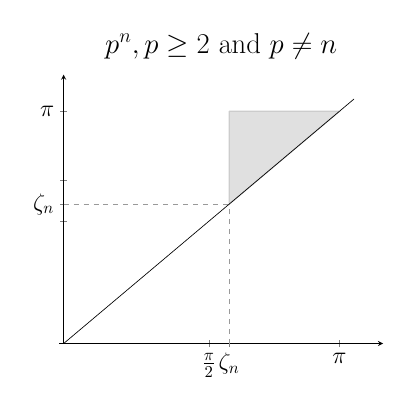
\begin{tikzpicture}[scale=0.6]
			\begin{axis} [
				title = {\LARGE $\Hbarc{p}{\bbS^n}, p\geq 2$ and $p\neq n$},
				ticklabel style = {font=\Large},
				axis y line=middle,
				axis x line=middle,
				ytick={0.5,0.57,0.67,0.95},
				yticklabels={,$\zeta_n$,,$\pi$},
				xtick={0.5,0.57,0.95},
				xticklabels={$\frac{\pi}{2}$,$\zeta_n$, $\pi$},
				xmin=-0.015, xmax=1.1,
				ymin=0, ymax=1.1,]
				\addplot [thick,color=black!20!white,fill=black!30!white,
				fill opacity=0.4]coordinates {
					(0.57,0.95)
					(0.57,0.57)
					(0.95,0.95)
					(0.57,0.95)};
				\addplot [black!40!white,mark=none,dashed, thin] coordinates {(0,0.57) (0.57,0.57)};
				\addplot [black!40!white,mark=none,dashed, thin] coordinates {(0.57,0) (0.57,0.57)};
				\addplot [mark=none] coordinates {(0,0) (1,1)};
			\end{axis}
		\end{tikzpicture}
	\end{tabular}
	\caption{Barcodes of $\bbS^n$, for $n\geq 2$ and degrees $p\geq 2$. Here, $\zeta_n=\arccos(-\frac{1}{n+1})$.
		In each figure, the gray area represents the only region, apart from the blue dots, where points could potentially exist within the corresponding barcode.}
	\label{fig:Sk}
\end{figure}

We study the Steenrod barcodes of $\bbS^n$. For any $k\in \Z_{\geq 1}$, the Steenrod square operation $\Sq^k$ is trivial for $\bbS^n$. Combined with Proposition \ref{prop:homotopy type} (\ref{prop:Sn}), we conclude that no Steenrod bars can be born before $\zeta_n$. Thus, all bars in $\sqbarc{k}{\bbS^n}$ are those dominated by  $(\zeta_n,\pi)$.

\subsection{Wedge sums}

The wedge sum $(X_1,x_1)\vee (X_2,x_2)$ (or simply $X_1\vee X_2$) of two pointed metric spaces $(X_1,x_1)$ and $(X_2,x_2)$ is the quotient space of the disjoint union of $X_1$ and $X_2$ by the identification of basepoints $x_1\sim x_2$.
Recall from \cite{burago2001course} that the \emph{gluing metric} on $X_1\vee X_2$ is given by \label{para:gluing}: %\facundo{Shouldn't cite Adams et al for this! They did not invent the glueing metric!!}
$$d_{X_1\vee X_2}(x_1',x_2')\defeq d_{X_1}(x_1',x_1)+d_{X_2}(x_2',x_2),\forall x_1'\in X_1, x_2'\in X_2$$
and $d_{X_1\vee X_2}\vert_{X_1\times X_1}\defeq d_{X_1},d_{X_1\vee X_2}\vert_{X_2\times X_2}\defeq d_{X_2}$. Notice that the above definition can be generalized to the case when we glue $n$ pointed metric spaces $(X_1,x_1),\cdots,(X_n,x_n)$ by identifying $x_i\sim x_j$ for all $1\leq i,j\leq n$. We denote the resulting space by $\bigvee_{i=1}^n (X_i,x_i)$, or $\bigvee_{i=1}^n X_i$ for simplicity, with the gluing metric:
$$d_{\bigvee_{i=1}^n X_i}(x_i',x_j')\defeq d_{X_i}(x_i',x_i)+d_{X_j}(x_j',x_j),\forall i\neq j, x_i'\in X_i, x_j'\in X_j$$
and $d_{X_i\vee X_i}|_{X_i\times X_i}\defeq d_{X_i}$ for any $1\leq i\leq n$.\\


Recall from \cite[Proposition 3.7]{adamaszek2020homotopy} that the Vietoris--Rips complex of a metric gluing is homotopy equivalent to the wedge sum of the Vietoris--Rips complexes. From this, we deduce the following proposition. \facundo{A priory, parameter wise homotphy equivalences do not guarantee same barcodes. One has to have some commutativity. See paper with Osman and Sunhyuk.}
\ling{I have added the reference}

\begin{proposition}\label{prop:wedge sum}
	Let $X$ and $Y$ be two compact metric spaces.
	\begin{enumerate}[(a)]
		\item\label{prop:wedge sum pH} For any degree $p$,
		\begin{equation*}\label{eq:wedge sum pH}
			\Hbarc{p}{X\vee Y}= \Hbarc{p}{X}\sqcup \Hbarc{p}{Y}.
		\end{equation*}
		\item\label{prop:wedge sum Sq} For any $k\in \Z_{\geq 1}$,
		\begin{equation*}\label{eq:wedge sum Sq}
			\sqbarc{k}{X\vee Y}= \sqbarc{k}{X}\sqcup \sqbarc{k}{Y}.
		\end{equation*}
	\end{enumerate}
\end{proposition}
\begin{proof}
	Item (\ref{prop:wedge sum pH}) follows from \cite[Proposition 3.7]{adamaszek2020homotopy} and \cite[Thoerem 9 (2)]{lim2020vietoris}.

	\ling{add the proof of Item (\ref{prop:wedge sum Sq}).}
\end{proof}

\subsection{Barcodes and Steenrod barcodes of $\bbS^1\vee\bbS^2\vee\dots\vee\bbS^n$}

Using Example \ref{ex:Sn} and Proposition \ref{prop:wedge sum} (\ref{prop:wedge sum pH}), we obtain (an estimate of) the barcodes of $X_n\defeq \bbS^1\vee\bbS^2\vee\dots\vee\bbS^n$, illustrated in the top row of Figure \ref{fig:barcodes}:
\begin{itemize}
	\item $\Hbarc{1}{X_n}$ contains only one bar $\left(0,\frac{2\pi}{3}\right)$.
	\item For any degree $2\leq p\leq n$, $\Hbarc{p}{X_n}$ contains one bar $(0,\zeta_p)$, and possibly some bars dominated by $(\zeta_n,\pi)$. For instance, when $p=2l+1$ is odd, $\Hbarc{p}{X_n}$ contains the bar $( \frac{2l\pi}{2l+1},\frac{2(l+1)\pi}{2l+3})$ which is dominated by $(\zeta_n,\pi)$.
	\item For any degree $p>n$, all bars in $\Hbarc{p}{X_n}$ are dominated by $(\zeta_n,\pi)$.
\end{itemize}

Using Example \ref{ex:Sn} and Proposition \ref{prop:wedge sum} (\ref{prop:wedge sum Sq}), we see that all bars in the Steenrod barcodes of $X_n$ are dominated by $\cup_{1\leq i\leq n}(\zeta_i,\pi)=(\zeta_n,\pi)$, so they can be illustrated as in the top row of Figure \ref{fig:sq barcodes}.

\begin{figure}
	\centering
	\begin{tikzpicture}[scale=0.52]
		\begin{axis} [
			title = {\LARGE $\Hbarc{p}{X_n},1\leq p\leq n$},
			ticklabel style = {font=\Large},
			axis y line=middle,
			axis x line=middle,
			ytick={0.5,0.6,0.67,0.95},
			yticklabels={,$\zeta_p$,,$\pi$},
			xtick={0.5,0.55,0.95},
			xticklabels={$\frac{\pi}{2}$,$\zeta_n$, $\pi$},
			xmin=-0.015, xmax=1.1,
			ymin=0, ymax=1.1,]
			\addplot [mark=none] coordinates {(0,0) (1,1)};
			\addplot [thick,color=black!20!white,fill=black!30!white,
			fill opacity=0.4]coordinates {
				(0.55,0.95)
				(0.55,0.55)
				(0.95,0.95)
				(0.55,0.95)};
			\addplot [black!40!white,mark=none,dashed, thin] coordinates {(0,0.6) (0.6,0.6)};
			\addplot [black!40!white,mark=none,dashed, thin] coordinates {(0,0.55) (0.55,0.55)};
			\addplot [black!40!white,mark=none,dashed, thin] coordinates {(0.55,0) (0.55,0.55)};
			\addplot[barccolor,mark=*] (0, 0.6) circle (2pt) node[above right,barccolor]{\Large\textsf{1}};
			%\node[mark=none] at (axis cs:0.68,0.21){$\Hbarc{2}{X_n}$};
		\end{axis}
	\end{tikzpicture}
	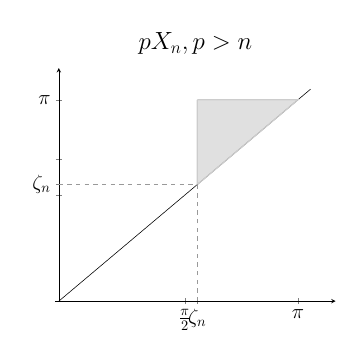
\begin{tikzpicture}[scale=0.52]
		\begin{axis} [
			title = {\LARGE $\Hbarc{p}{X_n}, p>n$},
			ticklabel style = {font=\Large},
			axis y line=middle,
			axis x line=middle,
			ytick={0.5,0.55,0.67,0.95},
			yticklabels={,$\zeta_n$,,$\pi$},
			xtick={0.5,0.55,0.95},
			xticklabels={$\frac{\pi}{2}$,$\zeta_n$, $\pi$},
			xmin=-0.015, xmax=1.1,
			ymin=0, ymax=1.1,]
			\addplot [mark=none] coordinates {(0,0) (1,1)};
			\addplot [thick,color=black!20!white,fill=black!30!white,
			fill opacity=0.4]coordinates {
				(0.55,0.95)
				(0.55,0.55)
				(0.95,0.95)
				(0.55,0.95)};
			\addplot [black!40!white,mark=none,dashed, thin] coordinates {(0,0.55) (0.55,0.55)};
			\addplot [black!40!white,mark=none,dashed, thin] coordinates {(0.55,0) (0.55,0.55)};
			%\node[mark=none] at (axis cs:0.68,0.21){$\Hbarc{p}{X_n}, p\geq 3$};
		\end{axis}
	\end{tikzpicture}

	\begin{tikzpicture}[scale=0.52]
		\begin{axis} [
			title = {\LARGE $\Hbarc{p}{\rp^n},1\leq p\leq n$},
			ticklabel style = {font=\Large},
			axis y line=middle,
			axis x line=middle,
			ytick={0.5,0.67,0.72,0.95},
			yticklabels={$\frac{\pi}{2}$,,$\frac{2\pi}{3}$,$\pi$},
			xtick={0.5,0.67,0.72,0.95},
			xticklabels={$\frac{\pi}{2}$,$\frac{2\pi}{3}$,,$\pi$},
			xmin=-0.015, xmax=1.1,
			ymin=0, ymax=1.1,]
			\addplot [mark=none] coordinates {(0,0) (1,1)};
			\addplot [thick,color=black!20!white,fill=black!30!white,
			fill opacity=0.4]coordinates {
				(0.67,0.95)
				(0.67,0.67)
				(0.95,0.95)
				(0.67,0.95)};
			\addplot [black!40!white,mark=none,dashed, thin] coordinates {(0,0.67) (0.67,0.67)};
			\addplot [black!40!white,mark=none,dashed, thin] coordinates {(0,0.72) (0.72,0.72)};
			\addplot [black!40!white,mark=none,dashed, thin] coordinates {(0.67,0) (0.67,0.67)};
			\addplot[barccolor,mark=*] (0, 0.72) circle (2pt) node[above right,barccolor]{\Large\textsf{1}};
			%\node[mark=none] at (axis cs:0.68,0.21){$\Hbarc{1}{\rp^n}$};
		\end{axis}
	\end{tikzpicture}
	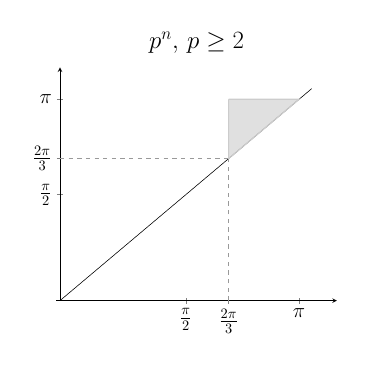
\begin{tikzpicture}[scale=0.52]
		\begin{axis} [
			title={\LARGE $\Hbarc{p}{\rp^n},\, p\geq 2$},
			ticklabel style = {font=\Large},
			axis y line=middle,
			axis x line=middle,
			ytick={0.5,0.67,0.95},
			yticklabels={$\frac{\pi}{2}$,$\frac{2\pi}{3}$,$\pi$},
			xtick={0.5,0.67,0.95},
			xticklabels={$\frac{\pi}{2}$,$\frac{2\pi}{3}$,$\pi$},
			xmin=-0.015, xmax=1.1,
			ymin=0, ymax=1.1,]
			\addplot [mark=none] coordinates {(0,0) (1,1)};
			\addplot [thick,color=black!20!white,fill=black!30!white,
			fill opacity=0.4]coordinates {
				(0.67,0.95)
				(0.67,0.67)
				(0.95,0.95)
				(0.67,0.95)};
			\addplot [black!40!white,mark=none,dashed, thin] coordinates {(0,0.67) (0.67,0.67)};
			\addplot [black!40!white,mark=none,dashed, thin] coordinates {(0.67,0) (0.67,0.67)};
			% \addplot[barccolor,mark=*] (0, 0.67) circle (2pt) node[above right,barccolor]{\Large\textsf{1}};
			% \node[mark=none] at (axis cs:0.68,0.21){$\Hbarc{p}{\rp^n},\, p\geq 2$};
		\end{axis}
	\end{tikzpicture}
	\caption{\emph{Top row:} barcodes of $X_n=\bbS^1\vee\bbS^2\vee\dots\vee\bbS^n$. \emph{Bottom row:} barcodes of $\rp^n$. }
	\label{fig:barcodes}
\end{figure}

\begin{figure}
	\centering
	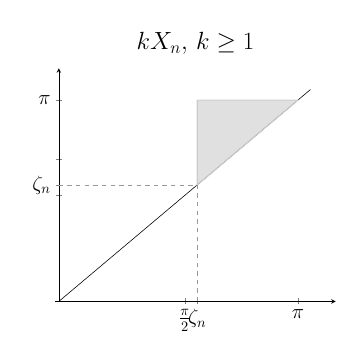
\begin{tikzpicture}[scale=0.52]
		\begin{axis} [
			title={\LARGE $\sqbarc{k}{X_n},\, k\geq 1$},
			ticklabel style = {font=\Large},
			axis y line=middle,
			axis x line=middle,
			ytick={0.5,0.55,0.67,0.95},
			yticklabels={,$\zeta_n$,,$\pi$},
			xtick={0.5,0.55,0.95},
			xticklabels={$\frac{\pi}{2}$,$\zeta_n$, $\pi$},
			xmin=-0.015, xmax=1.1,
			ymin=0, ymax=1.1,]
			\addplot [mark=none] coordinates {(0,0) (1,1)};
			\addplot [thick,color=black!20!white,fill=black!30!white,
			fill opacity=0.4]coordinates {
				(0.55,0.95)
				(0.55,0.55)
				(0.95,0.95)
				(0.55,0.95)};
			\addplot [black!40!white,mark=none,dashed, thin] coordinates {(0,0.55) (0.55,0.55)};
			\addplot [black!40!white,mark=none,dashed, thin] coordinates {(0.55,0) (0.55,0.55)};
			%\node[mark=none] at (axis cs:0.68,0.21){$\sqbarc{k}{X_n},\, k\geq 1$};
		\end{axis}
	\end{tikzpicture}

	\begin{tikzpicture}[scale=0.52]
		\begin{axis} [
			title = {\LARGE $\sqbarc{k}{\rp^n},\,1\leq k\leq n-1$},
			ticklabel style = {font=\Large},
			axis y line=middle,
			axis x line=middle,
			ytick={0.5,0.67,0.72,0.95},
			yticklabels={$\frac{\pi}{2}$,,$\frac{2\pi}{3}$,$\pi$},
			xtick={0.5,0.67,0.72,0.95},
			xticklabels={$\frac{\pi}{2}$,$\frac{2\pi}{3}$,,$\pi$},
			xmin=-0.015, xmax=1.1,
			ymin=0, ymax=1.1,]
			\addplot [mark=none] coordinates {(0,0) (1,1)};
			\addplot [thick,color=black!20!white,fill=black!30!white,
			fill opacity=0.4]coordinates {
				(0.67,0.95)
				(0.67,0.67)
				(0.95,0.95)
				(0.67,0.95)};
			\addplot [black!40!white,mark=none,dashed, thin] coordinates {(0,0.67) (0.67,0.67)};
			\addplot [black!40!white,mark=none,dashed, thin] coordinates {(0,0.72) (0.72,0.72)};
			\addplot [black!40!white,mark=none,dashed, thin] coordinates {(0.67,0) (0.67,0.67)};
			\addplot[barccolor,mark=*] (0, 0.72) circle (2pt) node[above right,barccolor]{\Large$\geq$\textsf{1}};
		\end{axis}
	\end{tikzpicture}
	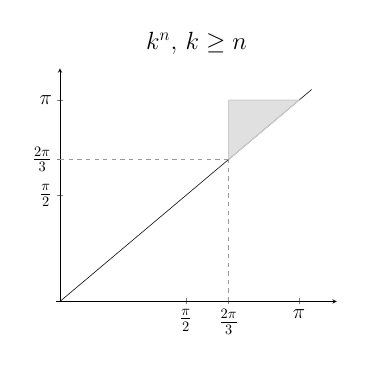
\begin{tikzpicture}[scale=0.52]
		\begin{axis} [
			title={\LARGE $\sqbarc{k}{\rp^n},\,k\geq n$},
			ticklabel style = {font=\Large},
			axis y line=middle,
			axis x line=middle,
			ytick={0.5,0.67,0.95},
			yticklabels={$\frac{\pi}{2}$,$\frac{2\pi}{3}$,$\pi$},
			xtick={0.5,0.67,0.95},
			xticklabels={$\frac{\pi}{2}$,$\frac{2\pi}{3}$,$\pi$},
			xmin=-0.015, xmax=1.1,
			ymin=0, ymax=1.1,]
			\addplot [mark=none] coordinates {(0,0) (1,1)};
			\addplot [thick,color=black!20!white,fill=black!30!white,
			fill opacity=0.4]coordinates {
				(0.67,0.95)
				(0.67,0.67)
				(0.95,0.95)
				(0.67,0.95)};
			\addplot [black!40!white,mark=none,dashed, thin] coordinates {(0,0.67) (0.67,0.67)};
			\addplot [black!40!white,mark=none,dashed, thin] coordinates {(0.67,0) (0.67,0.67)};
		\end{axis}
	\end{tikzpicture}
	\caption{\emph{Top row:} Steenrod barcodes of $X_n$. \emph{Bottom row:} Steenrod barcodes of $\rp^n$. }
	\label{fig:sq barcodes}
\end{figure}


\subsection{Barcodes and Steenrod barcodes of $\rp^n$}

Because the Vietoris--Rips complexes of $\rp^n$ are contractible when the scale parameter $t>\pi$, neither the standard barcodes nor the Steenrod barcodes can stay alive after $\pi$. Therefore, all bars are dominated by $(0,\pi)$.

For the standard barcodes of $\rp^n$, by applying Proposition \ref{prop:homotopy type} (\ref{prop:RPn}) and (\ref{prop:RPn bar}), %and the fact that $\opH_p(\rp^n;\,\Ftwo)$ is $\Ftwo$ for $p\leq n$ and $0$ otherwise,
we obtain the following:
\begin{itemize}
	\item For any $1\leq p\leq n$, $\Hbarc{p}{\rp^n}$ contains one bar $\left(0,\frac{2\pi}{3}\right)$ and possibly some bars  dominated by $\left(\frac{2\pi}{3},\pi\right)$.
	\item For $p>n$, all bars in $\Hbarc{p}{\rp^n}$ are dominated by $\left(\frac{2\pi}{3},\pi\right)$.
\end{itemize}

To compute the Steenrod barcodes of $\rp^n$, we first recall the following properties of $\rp^n$:
\begin{itemize}
	\item The cohomology ring $\opH^*\left(\rp^n;\,\Ftwo\right)$ is isomorphic to $\Ftwo[\alpha]/(\alpha^{n+1})$ (see \cite[Theorem 3.19]{hatcher2000});
	\item The Steenrod operations satisfy $\Sq^k(\alpha^m)=\left({m \choose k} \mod 2\right)\alpha^{m+k}$ for any $0\leq k\leq m\leq n$, according to Formula (*) on page 490 of \cite{hatcher2000}.
	\item For $k>\frac{n-1}{2}$, $\Sq^k\equiv 0$. Indeed, for $m\leq \frac{n-1}{2}<k$, it follows from \cite[page 489, Item (5)]{hatcher2000} that $\Sq^k(\alpha^m)=0$. For $m> \frac{n-1}{2}$, $\Sq^k(\alpha^m)=\left({m \choose k} \mod 2\right)\alpha^{m+k}=0$ because $m+k>n-1.$ Thus, $\Sq^k(\alpha^m)=0$ for any $m$.
	%For each $1\leq k\leq n-1$, let $k\leq m_k\leq n-1-k$ be such that ${m \choose k} \mod 2$
\end{itemize}
Let $1\leq k\leq \frac{n-1}{2}$. Since the Vietoris--Rips complex $\VR_t\left(\rp^n\right)$ retains the homotopy type of $\rp^n$ for $t\in \left(0,\frac{2\pi}{3}\right)$, we have at least one bar generated by $\Sq^k(\alpha^k)=\alpha^{2k}$ in the $\Sq^k$--barcode that is born at $0$ and stay alive until the non-trivial degree-$(k+1)$ class $\alpha^{2k}$ dies at $\frac{2\pi}{3}$. Therefore,
\begin{itemize}
	\item For $1\leq k\leq n-1$, $\sqbarc{k}{\rp^n}$ contains one bar $\left(0,\frac{2\pi}{3}\right)$, and possibly some bars dominated by $\left(\frac{2\pi}{3},\pi\right)$;
	\item For $k>n$, the possible bars in $\sqbarc{k}{\rp^n}$ are $\left(0,\frac{2\pi}{3}\right)$ or those dominated by $\left(\frac{2\pi}{3},\pi\right)$.
\end{itemize}


\subsection{Bottleneck distance estimation}

We estimate the bottleneck distance $\db$ between the Steenrod barcodes of the two space $X_n$ and $\rp^n$, and show that it provides a better (lower-bound) approximation of the Gromov-Hausdorff distance than $\db$ between the standard barcodes.

\begin{theorem}\label{prop:db estimate}
	\ \par
	\begin{itemize}
		\item[(1)] $\max_{p\geq 1}\db\left(\Hbarc{p}{X_n}, \Hbarc{p}{\rp^n}\right)\leq \frac{\pi-\zeta_n}{2}<\frac{\pi}{4}$.
		\smallskip\item[(2)] $\db\left(\sqbarc{k}{X_n}, \sqbarc{k}{\rp^n}\right)\geq \frac{\pi}{3},\forall 1\leq k\leq n-1$.
	\end{itemize}
\end{theorem}

\begin{proof}
	For Item (1), recall the barcodes of the two spaces from Figure \ref{fig:barcodes}, and note that to prove the bottleneck distance is upper bounded by $\frac{\pi-\zeta_n}{2}$, it is enough to find one matching with cost no larger than this value. Note that
	\[\frac{\pi}{2}<\zeta_n<\dots<\zeta_2<\zeta_1 =\frac{2\pi}{3}.\]

	For any degree $1\leq p\leq n$, consider a matching such that $(0,\zeta_p)\leftrightarrow \left(0,\frac{2\pi}{3}\right)$ and all other points are matched to the diagonal. The cost of this matching is at most
	\[\max\left\{\frac{2\pi}{3}-\zeta_p,\,\frac{\pi-\zeta_p}{2}\right\}.\]
	For degree $p>n$, consider a matching such that all points are matched to the diagonal, whose cost is at most $\max\left\{ \frac{\pi-\zeta_n}{2}, \frac{\pi-\frac{2\pi}{3}}{2}\right\} = \frac{\pi-\zeta_n}{2}<\frac{\pi}{4}.$ \\

	For Item (2), recall the Steenrod barcodes of the two spaces from Figure \ref{fig:sq barcodes}. For any $1\leq k\leq n-1$, the bar $\left(0,\frac{2\pi}{3}\right)$ in $\sqbarc{k}{\rp^n}$ can be mapped to either the diagonal or a point whose first coordinate is larger than or equal to $\zeta_n$. Therefore, a matching between the $\Sq^k$--barcodes will have a cost that is at least $\min\left\{\frac{1}{2}\cdot\frac{2\pi}{3}, \zeta_n\right\} = \frac{\pi}{3}.$
\end{proof}

Proposition \ref{prop:db estimate} shows that the Steenrod barcodes can have a stronger distinguishing power than the standard barcodes in all degrees.
